% ******************************************************** %
%              TEMPLATE DE INFORME ORGA2 v0.1              %
% ******************************************************** %
% ******************************************************** %
%                                                          %
% ALGUNOS PAQUETES REQUERIDOS (EN UBUNTU):                 %
% ========================================
%                                                          %
% texlive-latex-base                                       %
% texlive-latex-recommended                                %
% texlive-fonts-recommended                                %
% texlive-latex-extra?                                     %
% texlive-lang-spanish (en ubuntu 13.10)                   %
% ******************************************************** %


\documentclass[a4paper]{article}
\usepackage[spanish]{babel}
\usepackage[utf8]{inputenc}
\usepackage{charter}   % tipografia
\usepackage{graphicx}
%\usepackage{makeidx}
\usepackage{paralist} %itemize inline

%\usepackage{float}
\usepackage{amsmath, amsthm, amssymb}
\usepackage{amsfonts}
%\usepackage{sectsty}
%\usepackage{charter}
%\usepackage{wrapfig}
\usepackage{listings}
\lstset{language=C}

% \setcounter{secnumdepth}{2}
\usepackage{underscore}
\usepackage{caratula}
\usepackage{url}


% ********************************************************* %
% ~~~~~~~~              Code snippets             ~~~~~~~~~ %
% ********************************************************* %

\usepackage{color} % para snipets de codigo coloreados
\usepackage{fancybox}  % para el sbox de los snipets de codigo

\definecolor{litegrey}{gray}{0.94}

\newenvironment{codesnippet}{%
	\begin{Sbox}\begin{minipage}{\textwidth}\sffamily\small}%
	{\end{minipage}\end{Sbox}%
		\begin{center}%
		\vspace{-0.4cm}\colorbox{litegrey}{\TheSbox}\end{center}\vspace{0.3cm}}



% ********************************************************* %
% ~~~~~~~~         Formato de las páginas         ~~~~~~~~~ %
% ********************************************************* %

\usepackage{fancyhdr}
\pagestyle{fancy}

%\renewcommand{\chaptermark}[1]{\markboth{#1}{}}
\renewcommand{\sectionmark}[1]{\markright{\thesection\ - #1}}

\fancyhf{}

\fancyhead[LO]{Sección \rightmark} % \thesection\
\fancyfoot[LO]{\small{Agustín Borgna, Alan Corleto, Franco Lancioni}}
\fancyfoot[RO]{\thepage}
\renewcommand{\headrulewidth}{0.5pt}
\renewcommand{\footrulewidth}{0.5pt}
\setlength{\hoffset}{-0.8in}
\setlength{\textwidth}{16cm}
%\setlength{\hoffset}{-1.1cm}
%\setlength{\textwidth}{16cm}
\setlength{\headsep}{0.5cm}
\setlength{\textheight}{25cm}
\setlength{\voffset}{-0.7in}
\setlength{\headwidth}{\textwidth}
\setlength{\headheight}{13.1pt}

\renewcommand{\baselinestretch}{1.1}  % line spacing

% ******************************************************** %


\begin{document}


\thispagestyle{empty}
\materia{Organización del Computador II}
\submateria{Segundo Cuatrimestre de 2014}
\titulo{Trabajo Práctico II}
\subtitulo{subtitulo del trabajo}
\integrante{Borgna, Agustín}{079/15}{aborgna@dc.uba.ar}
\integrante{Corleto, Alan}{XXX/XX}{mail}
\integrante{Lancioni, Franco}{XXX/XX}{mail}

\maketitle
\newpage

\thispagestyle{empty}
\vfill
\begin{abstract}
En el presente trabajo se describe la problemática de ...
\end{abstract}

\thispagestyle{empty}
\vspace{3cm}
\tableofcontents
\newpage


\normalsize
\newpage
\section{Objetivos generales}

El objetivo de este Trabajo Práctico es experimentar con sets de instrucciones SIMD de Intel ASM x86 sobre una serie de implementaciones de filtros en imágenes de mapas de bits (RGBA) con el propósito de entender mejor el rol del paralelismo de datos en este tipo de implementaciones y qué tan remunerador es. 
A partir de cada filtro, se plantearán implementaciones en C, SSE \footnote{Streaming SIMD Extensions} (set de instrucciones sobre registros de 128 bits), AVX \footnote{Advanced Vector Extensions} (también sobre 128 bits pero permitiendo operaciones en formato 'no-destructivo' \footnote{Preservan los operandos fuente}) y su expansión de 256 bits AVX2.	 Acompañadas todas de un análisis para poder contrastar y discutir su rendimiento.



\section{Contexto}

hi

\begin{figure}
  \begin{center}
	
\includegraphics[width=0.5\textwidth]{img/logouba.jpg}
	\caption{Descripcion de la figura}
	\label{nombreparareferenciar}
  \end{center}
\end{figure}


\paragraph{\textbf{Titulo del parrafo} } Bla bla bla bla.
Esto se muestra en la figura~\ref{nombreparareferenciar}.



\begin{codesnippet}
\begin{verbatim}

struct Pepe {

    ...

};

\end{verbatim}
\end{codesnippet}


\newpage
\section{Cropflip}

\subsection{Descripción}
La imagen destino del filtro consiste en invertir verticalmente (flip) un recorte (crop) de la imagen fuente a partir de offsets dados como parámetro. El ancho y alto en píxeles de la imagen destino también se pasa como parámetros.
La descripción matemática está dada por la fórmula:

$$ O_{i,\ j}^{k}=I_{tamy+offsety-i-1, \ \ offsetx+j}^{k} $$

Donde el 'crop' de la imagen input corresponde con los píxeles del tipo:

$$
I_{offsety+i, \ \ offsetx+j}^{k} 
\qquad \text{con} \quad 0 \leq i < tamy \ \ \ 0 \leq j < tamx 
$$

\begin{table}[h]
\centering
\mem
\begin{tabular}{l|c|c|c|c|c|c|l}
 & \multicolumn{1}{l|}{}      & \multicolumn{1}{l|}{}       & \multicolumn{1}{l|}{}       & \multicolumn{1}{l|}{}       & \multicolumn{1}{l|}{}       & \multicolumn{1}{l|}{}      &  \\ \hline
 & \cellcolor[HTML]{FFCB2F}$I_{30}$ & \cellcolor[HTML]{FFCB2F}$I_{31}$  & \cellcolor[HTML]{FD6864}$I_{32}$  & \cellcolor[HTML]{FD6864}$I_{33}$  & \cellcolor[HTML]{FD6864}$I_{34}$  & \cellcolor[HTML]{FD6864}$I_{35}$ &  \\ \hline
 & \cellcolor[HTML]{FFCB2F}$I_{24}$ & \cellcolor[HTML]{FFCB2F}$I_{25}$  & \cellcolor[HTML]{FD6864}$I_{26}$  & \cellcolor[HTML]{FD6864}$I_{27}$  & \cellcolor[HTML]{FD6864}$I_{28}$  & \cellcolor[HTML]{FD6864}$I_{29}$ &  \\ \hline
 & \cellcolor[HTML]{FFCB2F}$I_{18}$ & \cellcolor[HTML]{FFCB2F}$I_{19}$ & \cellcolor[HTML]{FD6864}$I_{20}$ & \cellcolor[HTML]{FD6864}$I_{21}$ & \cellcolor[HTML]{FD6864}$I_{22}$  & \cellcolor[HTML]{FD6864}$I_{23}$ &  \\ \hline
 & \cellcolor[HTML]{FFCB2F}$I_{12}$ & \cellcolor[HTML]{FFCB2F}$I_{13}$ & \cellcolor[HTML]{FD6864}$I_{14}$ & \cellcolor[HTML]{FD6864}$I_{15}$ & \cellcolor[HTML]{FD6864}$I_{16}$  & \cellcolor[HTML]{FD6864}$I_{17}$ &  \\ \hline
 & \cellcolor[HTML]{FFCB2F}$I_{6}$ & \cellcolor[HTML]{FFCB2F}$I_{7}$ & \cellcolor[HTML]{FFCB2F}$I_{8}$ & \cellcolor[HTML]{FFCB2F}$I_{9}$ & \cellcolor[HTML]{FFCB2F}$I_{10}$  & \cellcolor[HTML]{FFCB2F}$I_{11}$ &  \\ \hline
 & \cellcolor[HTML]{FFCB2F}$I_{0}$ & \cellcolor[HTML]{FFCB2F}$I_{1}$ & \cellcolor[HTML]{FFCB2F}$I_{2}$ & \cellcolor[HTML]{FFCB2F}$I_{3}$ & \cellcolor[HTML]{FFCB2F}$I_{4}$  & \cellcolor[HTML]{FFCB2F}$I_{5}$ &  \\ \hline
 & \multicolumn{1}{l|}{}      & \multicolumn{1}{l|}{}       & \multicolumn{1}{l|}{}       & \multicolumn{1}{l|}{}       & \multicolumn{1}{l|}{}       & \multicolumn{1}{l|}{}      &
\end{tabular}
\caption{Ilustracion de la imagen fuente en memoria. En rojo los pixeles del crop \newline
(offsetx = 2, offsety = 2, tamx = 4, tamy = 4)}
\end{table}

\begin{table}[h]
\centering
\mem
\begin{tabular}{l|c|c|c|c|l}
& \multicolumn{1}{l|}{}       & \multicolumn{1}{l|}{}   & \multicolumn{1}{l|}{}     & \multicolumn{1}{l|}{}      &  \\ \hline
 & \cellcolor[HTML]{FD6864}$I_{14}$ & \cellcolor[HTML]{FD6864}$I_{15}$ & \cellcolor[HTML]{FD6864}$I_{16}$  & \cellcolor[HTML]{FD6864}$I_{17}$ &  \\ \hline
 & \cellcolor[HTML]{FD6864}$I_{20}$ & \cellcolor[HTML]{FD6864}$I_{21}$ & \cellcolor[HTML]{FD6864}$I_{22}$  & \cellcolor[HTML]{FD6864}$I_{23}$ &  \\ \hline 
 & \cellcolor[HTML]{FD6864}$I_{26}$  & \cellcolor[HTML]{FD6864}$I_{27}$  & \cellcolor[HTML]{FD6864}$I_{28}$  & \cellcolor[HTML]{FD6864}$I_{29}$ &  \\ \hline
  & \cellcolor[HTML]{FD6864}$I_{32}$ & \cellcolor[HTML]{FD6864}$I_{33}$  & \cellcolor[HTML]{FD6864}$I_{34}$  & \cellcolor[HTML]{FD6864}$I_{35}$ &  \\ \hline
  & \multicolumn{1}{l|}{}       & \multicolumn{1}{l|}{}  & \multicolumn{1}{l|}{}      & \multicolumn{1}{l|}{}      &
\end{tabular}
\caption{Ilustracion de la imagen destino en memoria}
\end{table}




No es dificil notar que las filas del crop en la fuente no constituyen una tira contigua de píxeles en memoria, si no que se encuentran distanciadas por el tamaño en bytes de offsetx lo que implica que necesitaremos iterar en dos ciclos anidados para poder procesar el crop.

\subsection{Implementaciones}
Al no involucrar operaciones aritméticas entre componentes de la imagen, las implementaciones del filtro se centran en accesos a memoria. Por lo tanto, las implementaciones solamente difieren en el modo en que se copian y asignan píxeles a la imagen output, radicando en esos métodos nuestro foco de análisis. 
\subsubsection{Implementaciones C y SSE}
La implementación C simplemente se trata de recorrer la imagen con una sola variable aplicando pixel a pixel la transformación dada por la fórmula matemática previamente mencionada. Mientras que la implementación corresponiente a SSE recorre la imagen fuente desde la fila superior del recuadro ($I_{32}$ en el cuadro 1) del crop hacia abajo de a 4 píxeles por iteración como indica el siguiente pseudo-código: 


\begin{codesnippet}
\begin{verbatim}

temp = src + offsetx*4 +srcRowSize*(offsety+tamy-1)       
{Apunta al primer píxel de la esquina superior izq. del crop}
for i = 0 to tamy:  
--> for j = 0 to tamx:  
-----> xmm0 = [temp]
-----> [dst] = xmm0 
-----> dst = dst  + 16 
-----> temp =  temp + 16 
-----> temp = temp - (dstRowSize + srcRowSize)       
{Decrece el ancho de la imagen destino y el de la fuente para apuntar primer pixel de la fila de
abajo a la que procesó}    
--> end for 
end for 

\end{verbatim}
\end{codesnippet}



De esta manera, las lecturas y escrituras en memoria representan $\frac{1}{16} = 0,0625 =  6,25\%$ del total de los accesos a memoria de la implementación C.


\subsubsection{Implementaciones SIMD paralelo en 128 y 256 bits}
Se diferencian de la implementación anterior de SSE en el uso de la mayor cantidad posible de registros \xmm{} (\ymm{} de 256 bits en el caso de las implementaciones de AVX) para las operaciones de transferencia de bloques de pixeles de la imagen fuente a la destino. 
\\

Dado que las lecturas y escrituras en memoria de cada registro son independientes entre sí, la ejecución fuera de orden del procesador hace que la transferencia por bloque sea más rápida que la implementación individual (que recorre la imagen con un único registro \xmm{}). Por cuestiones de vecindad espacial de los píxeles en la memoria, los accesos a memoria de cada registro tienen chances particularmente altas de hit en caché, no demorando así las lecturas del resto de los registros.
\\

Recordando que los registros de AVX tienen 32 bytes de capacidad y cada píxel en nuestro formato ocupa 4 bytes, cada registro \ymm{} tendrá capacidad para:

$$ \frac{32 \ bytes}{4 \ \frac{bytes}{px}} = 8 \ px $$

Por lo cual, suponiendo $ tamx \equiv 0 \ (mod \ 8) $ (como es el caso de una imagen de salida de 512x512), tendríamos $\frac{1}{32} = 0,03125 =  3,125\%$ del total de accesos a memoria de la implementación en C.

\subsubsection{Copiado paralelo de vectores}
\label{explicacionCopyN}

La asignación de píxeles se hace llamando a las funciones externas 'copyN_sse' y 'copyN_avx2'\footnote{../entregable/tp2-bundle.v1/codigo/lib} que copian tiras de píxeles de una imagen a otra por bloques de 64/4/1 ó 128/8/1 píxeles (sse y avx2 respectivamente) según sea posible en cada iteración. A modo de ejemplo (los otros casos son análogos), para copiar bloques de 64px (256B) desde la posición indicada por rsi a la indicada por rdi se cargan los valores correspondientes de la siguiente manera:
\newline
\\
\xmm{0} $\leftarrow$ {[rsi]} \\
\xmm{1} $\leftarrow$ {[rsi+16]} \\
... \\
\xmm{14} $\leftarrow$ {[rsi+224]}  \\
\xmm{15} $\leftarrow$ {[rsi+240]} \\
\\
{[rdi]} $\leftarrow$ \xmm{0} \\
{[rdi+16]} $\leftarrow$ \xmm{1} \\
... \\
{[rdi+224]} $\leftarrow$ \xmm{14} \\
{[rdi+240]} $\leftarrow$ \xmm{15} \\

Esta técnica de aplicar por cada iteración operaciones que, comunmente, se harían en varias se conoce como 'loop unrolling'. Como desventaja frente a la optimización por paralelismo y minimización branch mispredictions, en códigos de mucho mayor tamaño podría aumentar tan significativamente el tamaño del binario que aumente fuertemente el número de 'cache misses'. En nuestro caso copyN.o (que incluye a 'copyN_sse' y 'copyN_avx2') pesa 3,3 kB y es bastante probable que entre enteramente en caché.
\\

En el caso del filtro Cropflip, las tiras de píxeles corresponden a tiras de tamaño 'tamx' (es decir, al ancho del crop).  


\subsection{Experimentos - Rendimiento y análisis}

\subsubsection{Comparación entre implementaciones}

\begin{figure}[h]
\centering
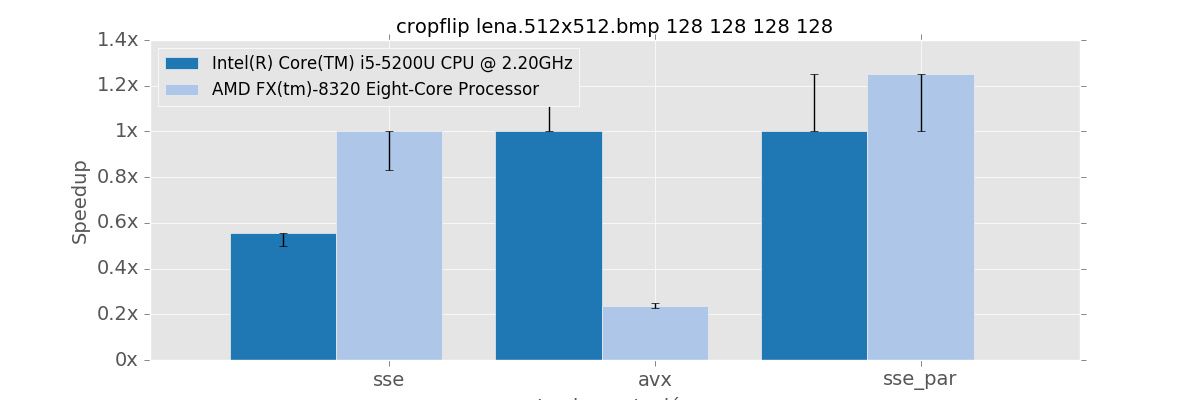
\includegraphics[width=0.90\textwidth]{cropflip-time-speedup} 
\caption{Tiempo de ejecución relativo de implementaciones ASM de cropflip contra la implementación C compilada con -O3}
\label{fig:cropflip-time-speedup}
\end{figure}

A diferencia de los otros dos filtros, donde el procesamiento de imágenes involucra operaciones aritméticas paralelas, la implementación AVX de	 Cropflip casi no presenta 'speedup' respecto de las implementaciones de SSE con registros de 128 bits en paralelo. 
\\

Sí se presentan entre las dos implementaciones de SSE, donde la diferencia es casi del doble a favor de SSE 'paralela'. Dados los parámetros tales que el recuadro de crop mide 128x128px, en la implementación con loop unrolling alcanza con dos iteraciones procesando 64px en cada una para cubrir cada fila. Mientras que para la versión SSE común hay que recorrer: $\frac{128 \ \frac{px}{fila}}{8 \ \frac{px}{iteracion}} = 32 \ \frac{iteraciones}{fila}$ .
\\

Sin embargo, la cantidad de iteraciones no refleja el hecho de que aún en ejecución fuera de orden los accesos a memoria siguen siendo individuales, teniendo que 'resecuencializar' las instrucciones para acceder ordenadamente. Podría suponerse que es debido a esto que el speedup no es del orden de magnitud que sugerirían las respectivas iteraciones por fila.

\subsubsection{Caché misses}

\begin{figure}[H]
\centering
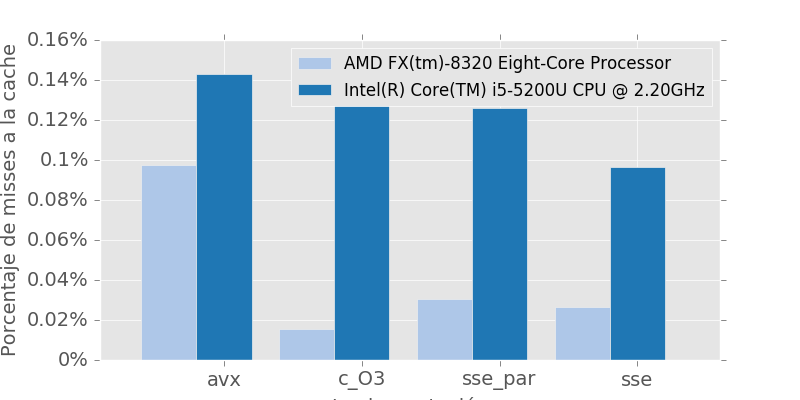
\includegraphics[width=0.90\textwidth]{cropflip-cache-misses}
\caption{Porcentaje de misses de la cache en la ejecución del filtro cropflip}
\label{fig:cropflip-cache-misses}
\end{figure}

\begin{figure}[H]
\centering
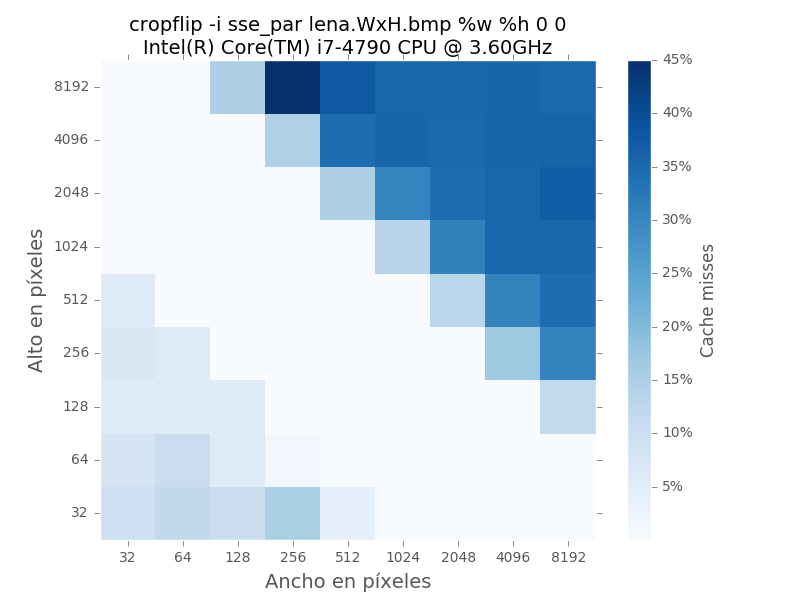
\includegraphics[width=0.7\textwidth]{cropflip-cache-map-sse-par-gflan-MS-7817}
\caption{Porcentaje de misses de la cache en función del tamaño de imagen durante la ejecución del filtro cropflip en la implementación SSE_paralelo}
\label{fig:cropflip-cache-map-sse_par-gflan-MS-7817}
\end{figure}

\subsubsection{Ciclos de Clock y Tiempo de ejecución - ASM y C}

Como habíamos anticipado al hablar del loop unrolling en SSE, el tamaño del binario no es lo suficientemente grande como para no poder ser cacheado eficientemente. La vecindad espacial de las tiras de píxeles también colaboran para que el hitrate se mantenga alto aún cuando las filas del crop no son contiguas en memoria como comentamos en la descripción. 

\begin{figure}[h]
\centering
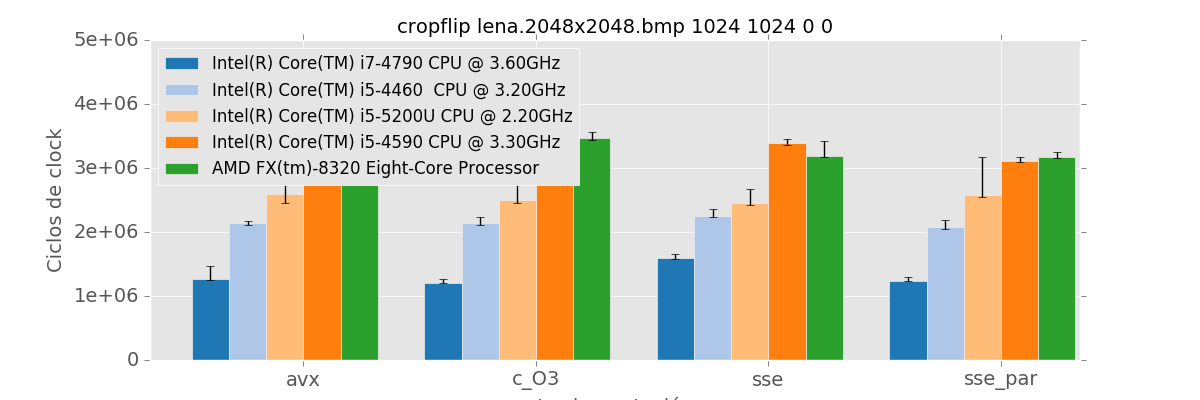
\includegraphics[width=0.90\textwidth]{cropflip-cycles} 
\label{fig:cropflip-cycles}
\end{figure}



Se observa una diferencia de casi la mitad ciclos de clock entre las versiones de SSE a favor del loop unrolling ('SSE Parelo') donde parecería que, gracias a un buen hitrate, los puntos fuertes  (particularmente paralelismo, no tanto minimizar branch mispredictions como veremos más adelante) destacan a pesar del hecho de que los accesos a memoria son individuales y no pueden solaparse.
\\

Pudimos corrobar que no es casualidad que el rendimiento de la implementación en C@-O3 sea similar al de las implementaciones SSE (particularmente 'SSE paralelo') utilizando GDB para ver el código compilado y comprobando que vectorizaba con operaciones SSE como se muestra a continuación:

\begin{figure}[H]
\centering
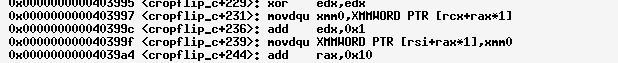
\includegraphics[width=0.90\textwidth]{untitled}
\end{figure}

A modo comparativo también incluímos el análisis de rendimiento entre las diversas optimizaciones para la implementación de C.

\begin{figure}[H]
\centering
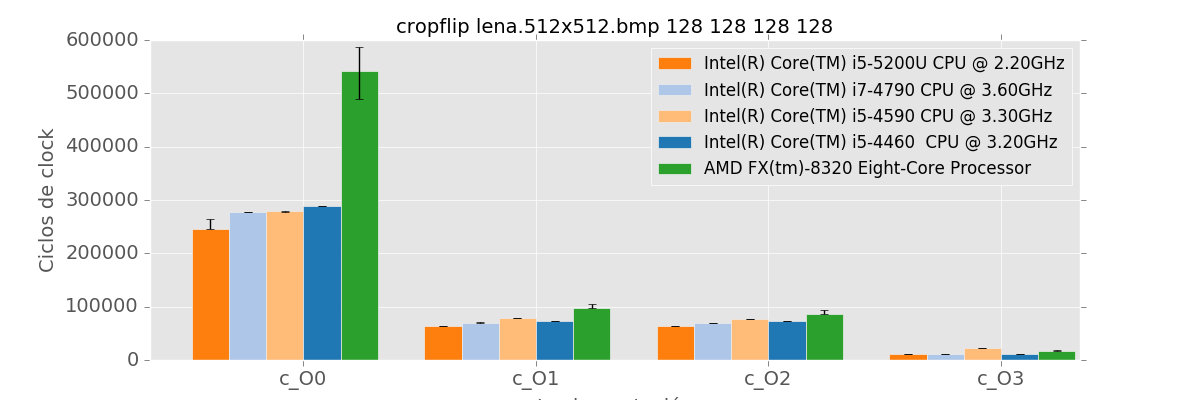
\includegraphics[width=0.90\textwidth]{cropflip-c-cycles} 
\label{fig:cropflip-c-cycles}
\end{figure}

\begin{figure}[H]
\centering
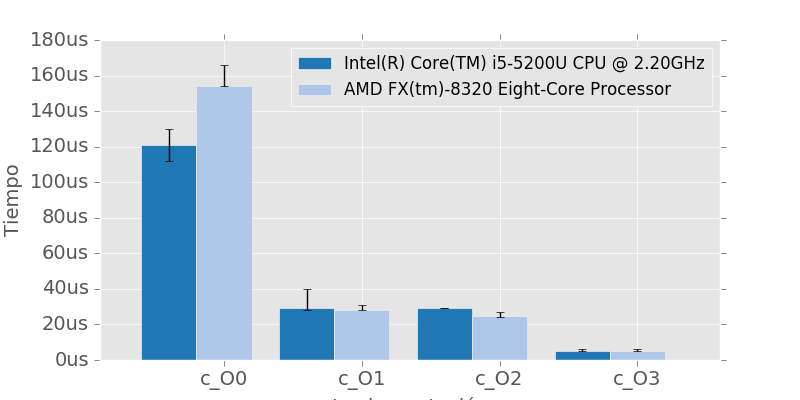
\includegraphics[width=0.90\textwidth]{cropflip-c-time} 
\label{fig:cropflip-c-time}
\end{figure}

\begin{figure}[H]
\centering
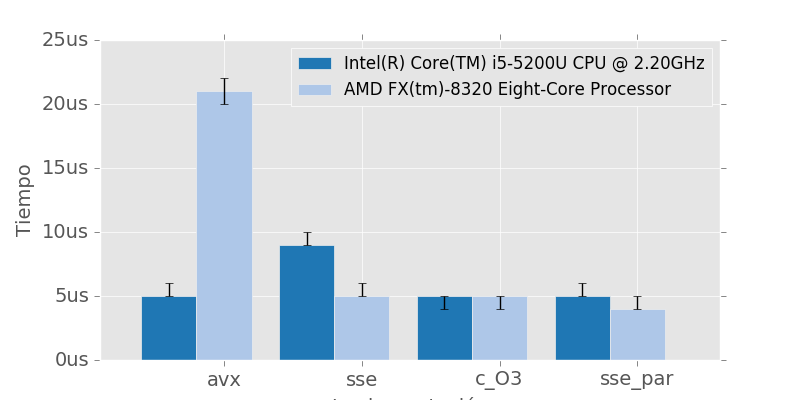
\includegraphics[width=0.90\textwidth]{cropflip-time}
\label{fig:cropflip-time}
\end{figure}

También es remarcable lo masivo que es el salto en rendimiento que se produce entre versiones de ASM y de C con optimización menor a -O3, donde bajan del rango de 20-160 microsegundos para las implementaciones C-O1/C-O2 a 3-8 microsegundos para las de ASM y C-03 (y cercanos al 10 por ciento para los rangos de ciclos de clock de las versiones de ASM vs C). Aún así, no parece verdaderamente remunerador para código centrado en accesos a memoria la elección de ASM frente al código C compilado con -O3.  

\begin{figure}[H]
\centering
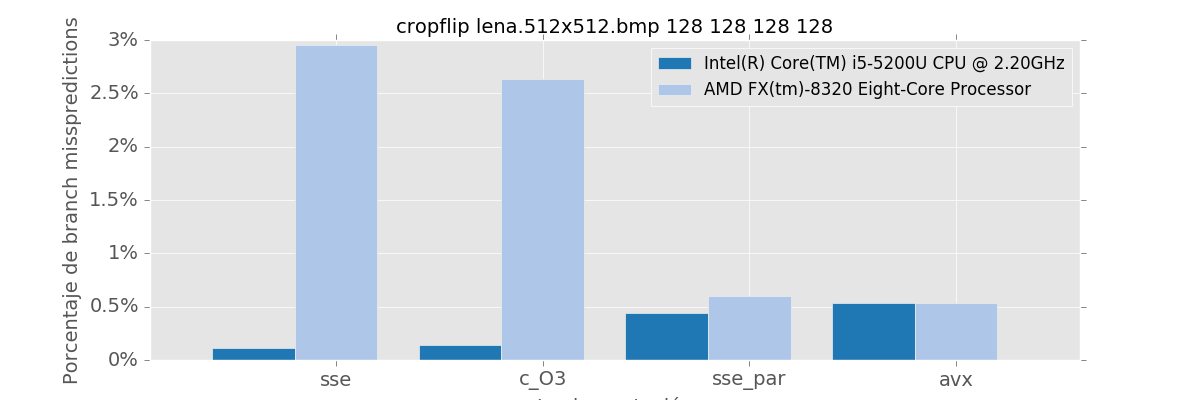
\includegraphics[width=0.90\textwidth]{cropflip-branch-misses}
\label{fig:cropflip-branch-misses}
\end{figure}

En este gráfico se puede apreciar algo bastante curioso: mientras que para algunos procesadores el loop unrolling minimizó muy efectivamente el porcentaje de branch mispredictions en las implementaciones de AVX y de SSE en paralelo frente a las implementaciones que procesan con un único vector (ya vimos que la implementación en C con optimización O3 también usa un registro XMM para los accesos a memoria), para otros significó un retroceso.
\ Esto resulta particularmente contraintuitivo si tenemos en cuenta que en teoría minimizar iteraciones parecería implicar minimizar predicciones y por lo tanto penalidades. Sin embargo esto se puede deber a que, en cada ciclo, se requiere evaluar si la cantidad restante de píxeles para copiar es mayor a  64/4/1 ó 128/8/1 píxeles para poder saltar a cada subrutina. Resultando así contraproducente desde este punto de vista dicha implementación.


\begin{figure}[H]
\centering
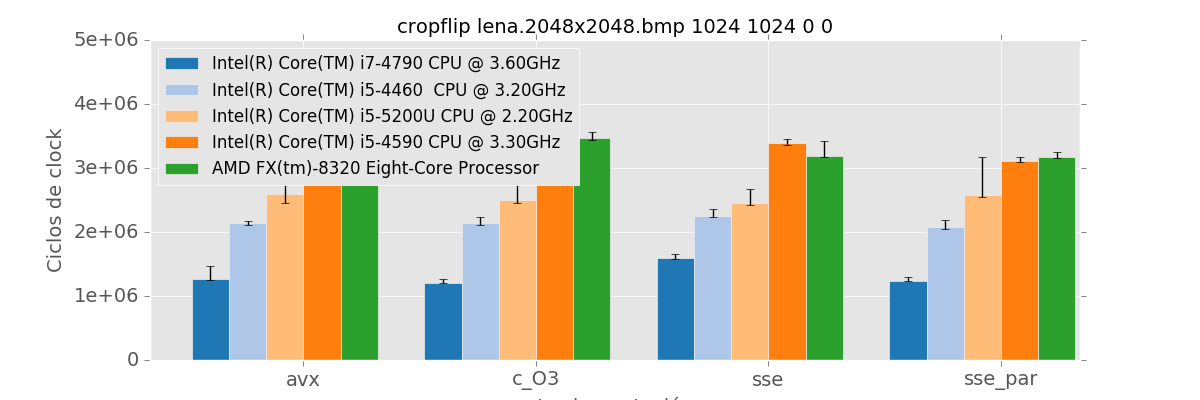
\includegraphics[width=0.90\textwidth]{cropflip-cycles}
\label{fig:cropflip-cycles}
\end{figure}




	

\newpage
\section{LDR (Low Dynamic Range)}

\subsection{Descripción}
 \cite{hackersdelight}
\subsection{Implementaciones}

\subsection{Experimentos}


\newpage
\section{Sepia}


\subsection{Descripción}

El filtro sepia consiste en cambiar los colores de cada pixel de la siguiente manera:

$$ O^r_{i,j} = 0,5 \cdot suma_{i,j} $$
$$ O^g_{i,j} = 0,3 \cdot suma_{i,j} $$
$$ O^b_{i,j} = 0,2 \cdot suma_{i,j} $$
$$ O^a_{i,j} = I^a_{i,j} $$

donde $suma_{i,j} = I^r_{i,j} + I^g_{i,j} + I^b_{i,j}$

Como puede verse, este filtro no recibe ningún parámetro y trabaja directamente con los datos mismos de la imagen.

\subsection{Implementaciones}

Antes de entrar en detalle a cada una de las implementaciones hechas, es importante notar que

$$suma_{i,j} = I^r_{i,j} + I^g_{i,j} + I^b_{i,j} \leq 255 + 255 + 255 = 3 \cdot 255$$

Lo cual excede el rango de representación de las componentes de un píxel. Esto puede resultar en un problema o no dependiendo de cada caso, ya que es necesario calcular $suma_{i,j}$ para resultados intermedios. Como el resultado final de aplicar el filtro en cada componente es multiplicar $suma_{i,j}$ por un número menor o igual a 1, se consideró aplicar la ley distributiva para poder salvar este problema, ya que, por ejemplo, en el caso de la componente azul

$$ O^b_{i,j} = 0,2 \cdot suma_{i,j} = 0,2 \cdot (I^r_{i,j} + I^g_{i,j} + I^b_{i,j}) = 0,2 \cdot I^r_{i,j} +  0,2 \cdot I^g_{i,j} + 0,2 \cdot I^b_{i,j} \leq 0,2 \cdot 255 + 0,2 \cdot 255 + 0,2 \cdot 255 = 0,6 \cdot 255 \leq 255$$


y en el caso de la componente verde

$$ O^b_{i,j} = 0,3 \cdot suma_{i,j} = 0,3 \cdot (I^r_{i,j} + I^g_{i,j} + I^b_{i,j}) = 0,3 \cdot I^r_{i,j} +  0,3 \cdot I^g_{i,j} + 0,3 \cdot I^b_{i,j} \leq 0,3 \cdot 255 + 0,3 \cdot 255 + 0,3 \cdot 255 = 0,9 \cdot 255 \leq 255$$

Cabe resaltar que realizando las operaciones de este modo, nunca se llega a un resultado intermedio el cual exceda el límite de representación de las componentes.

Sin embargo, esta alternativa fue descartada ya que implica hacer el triple de multiplicaciones en punto flotante, lo cual reduce drásticamente la performance.

Además, se debe notar que en el caso de la componente roja ocurre lo siguiente:

	$$ O^b_{i,j} = 0,5 \cdot suma_{i,j} \leq 0,5 \cdot 3 \cdot 255 = 1,5 \cdot 255$$

Lo cual resulta un problema a la hora de almacenar el resultado final ya que el mismo podría exceder el rango de representación de la componente roja. En cada una de las implementaciones se detalla cómo fue resuelta esta cuestión.

\subsubsection{C}

A grandes rasgos, la implementación en C es intuitiva, ya que recorre cada uno de los píxeles uno por uno, por cada iteración crea una variable auxiliar llamada $suma$ (la cual, como puede esperarse, contiene el valor de $suma_{i,j}$) y asigna a cada componente el valor de dicha suma multiplicada por su respectivo factor.
Debido a las dos problemáticas que se plantearon anteriormente, se hicieron algunos ajustes con respecto a la implementación. La variable auxiliar $suma$ es una variable del tipo $unsigned short (16 bits)$  para no perder precisión en las operaciones. Por la misma razón, se creó también una nueva variable auxiliar $suma_r$, la cual contiene el valor de $0,5 \cdot suma_{i,j} = I^r_{i,j}$.
Para volver a $char (8 bits)$ se resuelve distinto en cada caso.
\begin{itemize}
	\item En el caso de $suma$ con respecto a las componentes azul y verde, solamente se les asigna a cada una el valor de $suma$ multiplicado por su respectivo factor ya que, como se demostró anteriormente, $O^b_{i,j}$ y $O^g_{i,j}$ son siempre menores a 255 y por lo tanto no hay que tener ningún recaudo extra. Luego de ejecutar la multiplicación, el lenguaje C simplemente convierte el dato a $char$ y lo asigna.
	\item En el caso de $suma_r$, se pregunta primero si el resultado final dio mayor o igual a 255. Si eso es cierto, lo satura a 255. Caso contrario, lo deja como está. En esencia se está ejecutando un $min(I^r_{i,j},255)$.
\end{itemize}

La cantidad de operaciones de punto flotante por píxel en esta implementación es de $\frac{3op}{px}$.

\subsubsection{Asm - SSE}

Cada componente ocupa 1 byte y cada píxel tiene 4 componentes, por lo cual un píxel ocupa 4 bytes. Como los registros \xmm{} son de 16B, es posible procesar 4 píxeles en un solo registro simultáneamente.
Al inicio del loop, se copian 4 píxeles de la imagen fuente a \xmm{0} para empezar a procesar. Para simplificar la notación, se llamará $K_{i}$ a la componente K del pixel $i \in {0,1,2,3}$

\xmm{0} \xmmByte{$A_{3}$}{$R_{3}$}{$G_{3}$}{$B_{3}$}{$A_{2}$}{$R_{2}$}{$G_{2}$}{$B_{2}$}{$A_{1}$}{$R_{1}$}{$G_{1}$}{$B_{1}$}{$A_{0}$}{$R_{0}$}{$G_{0}$}{$B_{0}$}

Luego, se copia a \xmm{1} y \xmm{3} el contenido de \xmm{0} y se borran los alpha de los mismos

\xmm{1} \xmmByte{$0$}{$R_{3}$}{$G_{3}$}{$B_{3}$}{$0$}{$R_{2}$}{$G_{2}$}{$B_{2}$}{$0$}{$R_{1}$}{$G_{1}$}{$B_{1}$}{$0$}{$R_{0}$}{$G_{0}$}{$B_{0}$}

\xmm{3} \xmmByte{$0$}{$R_{3}$}{$G_{3}$}{$B_{3}$}{$0$}{$R_{2}$}{$G_{2}$}{$B_{2}$}{$0$}{$R_{1}$}{$G_{1}$}{$B_{1}$}{$0$}{$R_{0}$}{$G_{0}$}{$B_{0}$}

Se desempaquetan \xmm{1} y \xmm{3} de tal manera que \xmm{1} tenga la parte baja y \xmm{3} la parte alta. Ambos terminarían convirtiéndose en registros de words empaquetados. Esto se hace con el fin de poder luego ejecutar una suma horizontal de a word sin el riesgo de que el resultado quede fuera del rango de representación.

\xmm{1} \xmmWord{$0$}{$R_{1}$}{$G_{1}$}{$B_{1}$}{$0$}{$R_{0}$}{$G_{0}$}{$B_{0}$}

\xmm{3} \xmmWord{$0$}{$R_{3}$}{$G_{3}$}{$B_{3}$}{$0$}{$R_{2}$}{$G_{2}$}{$B_{2}$}

Se ejecutan las sumas horizontales necesarias para que \xmm{1} tenga el resultado

\xmm{1} \xmmWord{$0$}{$0$}{$0$}{$0$}{$S_{3}$}{$S_{2}$}{$S_{1}$}{$S_{0}$}

donde $S_{i} = R_{i} + G_{i} + B_{i}$

Se convierte \xmm{1} a float para poder realizar la multiplicación por los factores correspondientes, y luego se ejecutan varios shuffle de tal manera que haya un registro completo por cada píxel

\xmm{1} \xmmFloat{$S_{0}$}{$S_{0}$}{$S_{0}$}{$S_{0}$}

\xmm{2} \xmmFloat{$S_{1}$}{$S_{1}$}{$S_{1}$}{$S_{1}$}

\xmm{3} \xmmFloat{$S_{2}$}{$S_{2}$}{$S_{2}$}{$S_{2}$}

\xmm{4} \xmmFloat{$S_{3}$}{$S_{3}$}{$S_{3}$}{$S_{3}$}

Se multiplica a los cuatro registros por el siguiente vector de factores que se encuentra alojado en \xmm{15}

\xmm{15} \xmmFloat{$0$}{$0,5$}{$0,3$}{$0,2$}

Lo cual da como resultado

\xmm{1} \xmmFloat{$0$}{$0,5 \cdot S_{0}$}{$0,3 \cdot S_{0}$}{$0,2 \cdot S_{0}$}

\xmm{2} \xmmFloat{$0$}{$0,5 \cdot S_{1}$}{$0,3 \cdot S_{1}$}{$0,2 \cdot S_{1}$}

\xmm{3} \xmmFloat{$0$}{$0,5 \cdot S_{2}$}{$0,3 \cdot S_{2}$}{$0,2 \cdot S_{2}$}

\xmm{4} \xmmFloat{$0$}{$0,5 \cdot S_{3}$}{$0,3 \cdot S_{3}$}{$0,2 \cdot S_{3}$}

Es decir

\xmm{1} \xmmFloat{$0$}{$O^r_{0}$}{$O^g_{0}$}{$O^b_{0}$}

\xmm{2} \xmmFloat{$0$}{$O^r_{1}$}{$O^g_{1}$}{$O^b_{1}$}

\xmm{3} \xmmFloat{$0$}{$O^r_{2}$}{$O^g_{2}$}{$O^b_{2}$}

\xmm{4} \xmmFloat{$0$}{$O^r_{3}$}{$O^g_{3}$}{$O^b_{3}$}

Se reconvierte cada registro a int y se empaquetan de manera saturada los datos en \xmm{1}. La saturación es la solución al overflow de la componente roja, ya que la instrucción misma la transforma en 255 en caso de ser mayor.

\xmm{1} \xmmByte{$0$}{$O^r_{3}$}{$O^g_{3}$}{$O^b_{3}$}{$0$}{$O^r_{2}$}{$O^g_{2}$}{$O^b_{2}$}{$0$}{$O^r_{1}$}{$O^g_{1}$}{$O^b_{1}$}{$0$}{$O^r_{0}$}{$O^g_{0}$}{$O^b_{0}$}

Por el lado de \xmm{0}, se eliminan los datos de los colores y se deja solo el alpha para poder luego "fusionar" los datos con \xmm{1}

\xmm{0} \xmmByte{$A_{3}$}{$0$}{$0$}{$0$}{$A_{2}$}{$0$}{$0$}{$0$}{$A_{1}$}{$0$}{$0$}{$0$}{$A_{0}$}{$0$}{$0$}{$0$}

Por último, se unen los datos de \xmm{0} y \xmm{1} y se almacena en la imagen destino.

\xmm{0} \xmmByte{$O^a_{3}$}{$O^r_{3}$}{$O^g_{3}$}{$O^b_{3}$}{$O^a_{2}$}{$O^r_{2}$}{$O^g_{2}$}{$O^b_{2}$}{$O^a_{1}$}{$O^r_{1}$}{$O^g_{1}$}{$O^b_{1}$}{$O^a_{0}$}{$O^r_{0}$}{$O^g_{0}$}{$O^b_{0}$}

La cantidad de operaciones de punto flotante por píxel en esta implementación es de $\frac{4op}{4px} = \frac{1op}{px}$, La cual es menor comparado a la cantidad de operaciones por píxel de la implementación en C (la cual es $\frac{3op}{px}$).

\vspace{2mm}

Con la finalidad de aumentar el rendimiento de esta implementación, se decidió utilizar más registros para procesar más cantidad de memoria en un mismo loop, de modo tal que la ejecución fuera de orden fuera más efectiva y se realice la menor cantidad de saltos condicionales posible.

Como se pudo ver en el desarrollo del algoritmo, solo cinco registros fueron utilizados para realizar todo el proceso (\xmm{0}..\xmm{4}), esto nos permite procesar de a 12 píxeles por ciclo, utilizando 15 de los 16 registros xmm, dejando espacio libre para el registro extra que contiene los factores por los que hay que multiplicar.

También es necesario utilizar un registro lleno de ceros para desempaquetar los datos, lo cual haría necesario contar con 17 registros o acceder a memoria, pero como ese registro de ceros solo es necesario durante una sola parte del algoritmo (en la cual aún no están en uso todos los registros) se puede utilizar algún registro que aún no se haya procesado.

La problemática que surge a partir de procesar de a 12 píxeles, es que no se sabe si se puede estar procesando píxeles de más, ya que solo se tiene como hipótesis que el ancho de la imagen multiplicado por su altura es un número que es múltiplo de 8, y por ende no siempre tendremos una imagen cuyo tamaño total sea múltiplo de 12. Para solucionar esto, se procesa de a 12 píxeles todas las veces que se pueda, y cuando ya no se pueda más, se procesa de a 4 como originalmente se hacía, hasta terminar de procesar toda la imagen. Notar que no puede llegar a ocurrir que el algoritmo haya tenido que procesar de a 4 píxeles más de 2 veces.

\subsubsection{Asm - AVX2}

En AVX2 podemos utilizar los registros extendidos \ymm{} de 256 bits, por lo cual podemos procesar el doble de píxeles que en la implementación SSE. También contamos con instrucciones no destructivas que nos ahorran un par de pasos a la hora de implementar. Por ejemplo, podemos pasar de

\begin{lstlisting}
MOVDQA XMM1, XMM0
PSLLD XMM1, 8
PSRLD XMM1, 8
\end{lstlisting}

a

\begin{lstlisting}
VPSLLD XMM1, XMM0, 8
VPSRLD XMM1, XMM1, 8
\end{lstlisting}


La conversión del algoritmo es directa con respecto a SSE. La estrategia es la misma, con la salvedad de que hay que tener cuidado con algunas instrucciones que no funcionan exactamente igual a su instrucción análoga de SSE.

Por ejemplo, a la hora de convertir los registros a word ejecutando VPUNPCKLBW y VPUNPCKHBW, estos quedarían de la siguiente manera

\begin{lstlisting}
VPUNPCKLBW XMM3, XMM1, XMM7
VPUNPCKHBW XMM1, XMM1, XMM7
\end{lstlisting}

\ymm{1} \ymmWord{$0$}{$R_{5}$}{$G_{5}$}{$B_{5}$}{$0$}{$R_{4}$}{$G_{4}$}{$B_{4}$}{$0$}{$R_{1}$}{$G_{1}$}{$B_{1}$}{$0$}{$R_{0}$}{$G_{0}$}{$B_{0}$}

\ymm{3} \ymmWord{$0$}{$R_{7}$}{$G_{7}$}{$B_{7}$}{$0$}{$R_{6}$}{$G_{6}$}{$B_{6}$}{$0$}{$R_{3}$}{$G_{3}$}{$B_{3}$}{$0$}{$R_{2}$}{$G_{2}$}{$B_{2}$}

Por lo general, en las instrucciones de AVX2 se mantiene la misma estructura que se vio en el reciente ejemplo: Primero se procesa la parte baja de los dos registros fuente, y luego se procesa la parte alta de cada uno, en vez de procesar cada uno por completo a la vez.

Esta implementación ejecuta la misma cantidad de operaciones en punto flotante que SSE, pero procesa el doble de píxeles. Por lo tanto, por cada loop obtenemos un rendimiento de $\frac{4op}{8px} = \frac{1op}{2px}$.


\subsection{Experimentos}

\subsubsection{Comparación entre implementaciónes}

 Luego de realizar varias corridas de cada una de las implementaciones, se llegaron a los siguientes resultados en cuanto al tiempo total de ejecución:

\begin{figure}[h]
    \centering
    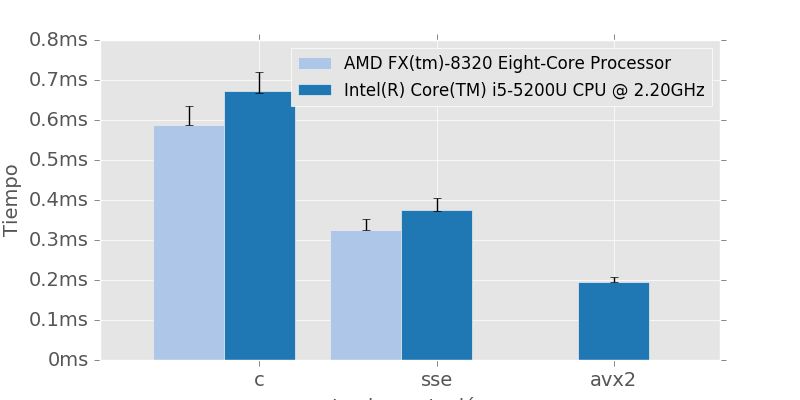
\includegraphics[width=0.9\textwidth]{sepia-time}
    \caption{Tiempo de ejecución del filtro sepia sobre lena.bmp 512x512}
    \label{fig:sepia-time}
\end{figure}

Se puede inferir entonces que las suposiciones anteriores en cuanto a mejoras de performance resultaron ser verdaderas. La implementación en SSE corre más rápido que la misma en C y la implementación en AVX2 corre aún más rápido que SSE.

En el siguiente gráfico se explicita con más detalle qué tanto más rápidas son las dos implementaciones en ASM con respecto a C compilado con la optimización O3:

\begin{figure}[h]
    \centering
    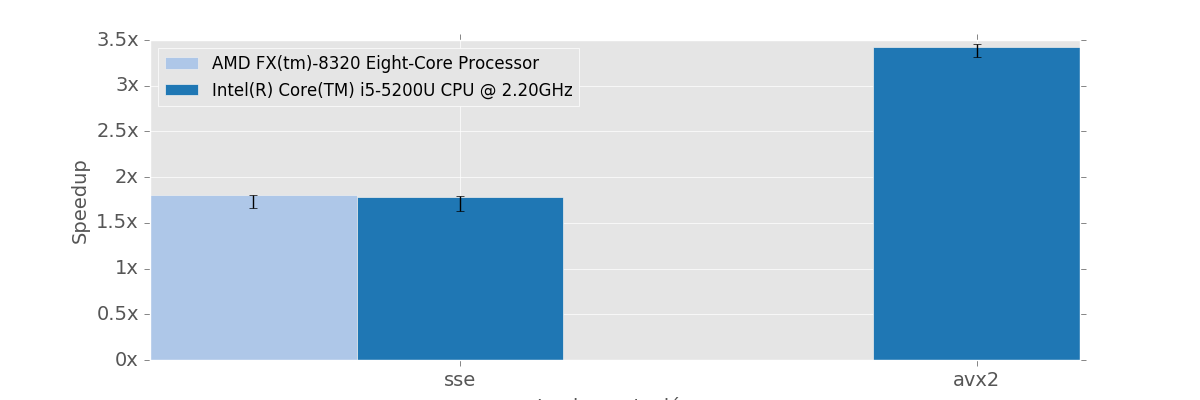
\includegraphics[width=0.9\textwidth]{sepia-time-speedup}
    \caption{Tiempo de ejecución relativo de implementaciones ASM de sepia contra la implementación C compilada con -O3}
    \label{fig:sepia-time-speedup}
\end{figure}

Se puede ver que SSE presenta un speedup de poco menos de 2 y AVX2 presenta un speedup de casi 3.5, evidenciando aún más fuertemente la mejora que se obtiene a medida que se va aumentando el paralelismo del procesamiento de píxeles.

Es importante aclarar que para realizar este experimento, se compiló la implementación en C con la opción de optimización automática O3.

\subsubsection{Comparación entre optimizaciones de C}

Las diferencias de performance entre la implementación C sin optimizar (O0) y las distintas optimizaciones se puede apreciar en el siguiente gráfico:

\begin{figure}[h]
    \centering
    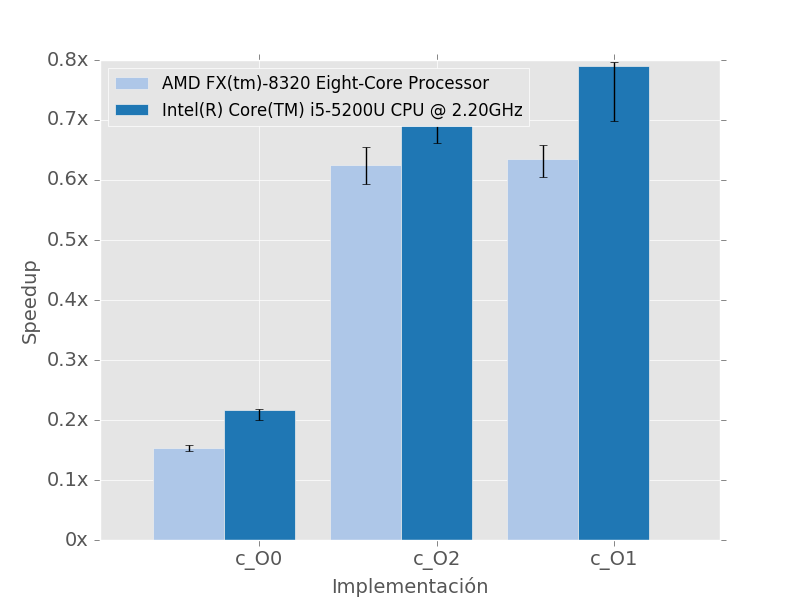
\includegraphics[width=0.9\textwidth]{sepia-c-time-speedup}
    \caption{Tiempo de ejecución relativo de diferentes optimizaciónes de la implementación en C respecto a lo optimización O3}
    \label{fig:sepia-c-time}
\end{figure}

Como puede verse, la versión sin optimizar es muchas veces más lenta que la versión completamente optimizada. Es decir que la diferencia entre la implementación en C sin optimizar y las implementaciones en SSE y AVX2 es aún más grande en cuanto a performance.

\subsubsection{Caché misses en función del tamaño de imagen}

Como siguiente cuestión, nos planteamos la pregunta sobre qué tanto porcentaje de Cache Misses se presentan al correr los códigos. Para encontrar una respuesta, decidimos hacer un experimento en el cual surgieron los siguientes resultados para la implementación en SSE:

\begin{figure}[h]
    \centering
    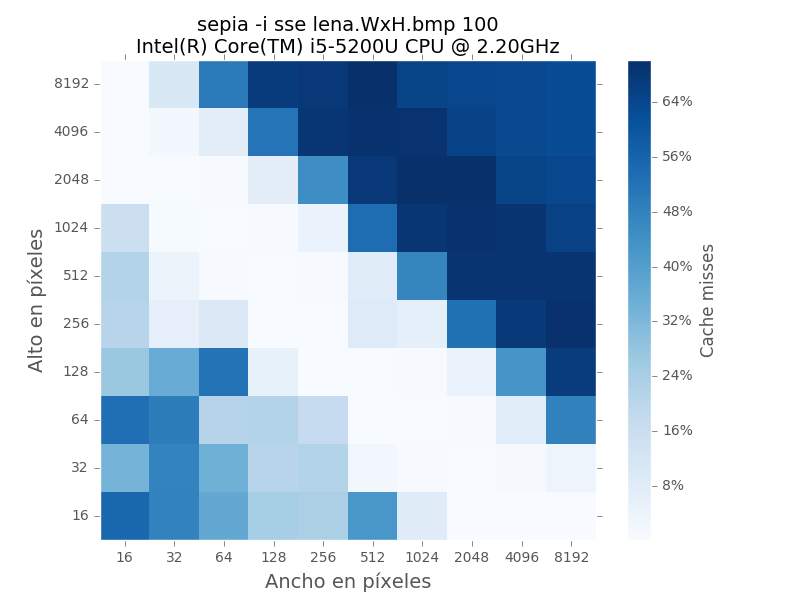
\includegraphics[width=0.65\textwidth]{sepia-cache-map-sse-angua}
    \caption{Porcentaje de caché misses en función del tamaño de imagen al correr el filtro sepia en un procesador con 3MB de caché}
    \label{fig:sepia-cache-map-sse-angua}
\end{figure}

Los casos que se encuentran alrededor de 128x128 tienen un miss rate ligeramente menor debido a que varios píxeles ya se encontraban en cache a la hora de volver a testear la misma imágen pero con distinto tamaño. Luego, al aumentar el ancho o el alto de la imagen, el miss rate va aumentando progresivamente ya que cada vez aumenta más la cantidad de datos que no estaban anteriormente en cache.

Es importante resaltar cómo se produce un cambio brusco de color en la diagonal que va de 4096x128 a 128x4096. Para poder explicar este fenómeno es necesario recalcar que el procesador con el cual se realizó este experimento posee 3MB de memoria cache. También hay que recordar que cada píxel ocupa 4B en memoria. Si realizamos algunas cuentas con cualquiera de los elementos de la diagonal antes mencionada:

$$(4096 \cdot 128) px = 2^{19} px = 2^{19} \cdot 4 B = 2 \cdot 2^{20} B = 2MB$$

Ahora que sabemos esto, tiene más sentido ver por qué a partir de que el tamaño total de la imagen es mayor o igual a $2^{19}$, comienza a haber un aumento considerable de cache misses, ya que la imagen misma comienza a no entrar en la cache entera. Si nos movemos a la siguiente diagonal (es decir, multiplicamos por 2 el tamaño de la imagen) estaríamos trabajando ya con casos que ocupan 4MB, lo cual es incluso mayor al tamaño de la cache con la que estamos trabajando. Por eso a partir de ese punto, todas las imágenes que tengan un tamaño mayor o igual poseen un miss rate bastante similar.

Esta misma estructura se repite para los casos de las implementaciones en C y en AVX2. Esa es la razón por la cual no incluimos también los gráficos para esos dos casos ya que presentan gráficos muy similares. La única diferencia es que el máximo miss rate en C es de $\sim80\%$ y en AVX es de $\sim60\%$. No sabemos bien por qué ocurre esto, pero suponemos que puede ser debido al tamaño de las lecturas. A medida que se procesan más píxeles por registro, menos lecturas hay que ejecutar.


\newpage
\section{Conclusiones y trabajo futuro}

Considerando los resultados de nuestros experimentos, creemos que la implementación de partes de un programa en assembler vale el esfuerzo cuando nuestro performance está limitado por una rutina que puede ser paralelizada. Ya que el tiempo que lleva programar en assembler es bastante mayor a lenguajes de mas alto nivel debemos considerar nuestros recursos antes de realizar todo el programa en asm.

En los filtros que realizaban cálculos logramos una gran mejora de performance al implementar usando la extensión AVX2 contra la versión SSE. Hay que tener mucho cuidado al usarla ya que varias instrucciones resultaron tener comportamientos diferentes a los que uno esperaría, sobre todo cuando se quiere hacer operaciones entre valores como un shuffle o una suma horizontal. De todos modos, leyendo cuidadosamente el manual y documentando bien cada paso se logran muy buenos resultados.
\\

Nos quedó en el tintero experimentar con flotantes de doble precisión y ver si podemos lograr precisiones exactas sin pagar la penalidad de las cuentas con enteros.

También querríamos constatar, ya que este año salen al mercado procesadores con la extensión AVX-512, si el aumento de rendimiento se mantiene mientras mas suba el tamaño de los registros, o nos encontraremos con demasiado overhead de los cálculos auxiliares.



\newpage
\bibliography{bibliography}{}
\bibliographystyle{plain}

\end{document}

